\chapter{(Finite) Markov Decision Processes \cite{medium-introduction-to-reinforcement-learning-rl-part-3-finite-markov-decision-processes-51e1f8d3ddb7}}

\section{Reinforcement Learning Recap}

% https://towardsdatascience.com/introduction-to-reinforcement-learning-rl-part-3-finite-markov-decision-processes-51e1f8d3ddb7

\begin{enumerate}
    \item The learner and decision-maker is called the \textbf{agent}.
    \item The thing it interacts with, comprising everything outside the agent, is called the \textbf{environment}.
    \item The agent interacts with the environment over a sequence of discrete \textbf{time steps}, $t = 0, 1, 2, 3, ...$
    \item At each time step $t$, the environment sends the agent a \textbf{state}, $S_t \in S$, where $S$ is the set of possible states.
    \item Based on that, the agent selects an \textbf{action}, $A_t \in A(S_t)$, where $A(S_t)$ is the set of actions available in state $S_t$.
    \item One time step later the agent receives a \textbf{reward}, $R_{t+1} \in R$, and finds itself in a new state, $S_{t+1}$.
    \item At each time step, the agent follows a mapping from its current state to probabilities of selecting each possible action in that state.
    \item This mapping is called the agent’s \textbf{policy} and is denoted $\pi_t(A \mid S)$, where $\pi_t(A \mid S)$ is the probability of taking action $A$ in state $S$ in time step $t$.
    \item The agent’s goal is to maximize the total reward it receives in the long run.
    \item we denote the sequence of rewards the agent receive after time step $t$ as: $R_{t+1}$, $R_{t+2}$, ...
    \item The agent seek to maximize the \textbf{expected return}: $E(G_t)$.
    \[
        G_t = R_{t+1} +R_{t+2} +R_{t+3} + \cdots + R_T
    \]
    where, $T$ is a final time step.
    \item when the agent’s and the environment’s interaction breaks naturally into subsequences (like playing chess, or TicTacToe), which we call \textbf{episodes}.
    \item Each episode ends in a special state called the \textbf{terminal state}. After the agent reach the terminal state, the game is reset to some starting state.
    \item Tasks with episodes of this kind are called \textbf{episodic tasks}.
    \item There are many situations where the interaction between the agent and the environment goes on continually without a limit (e.g a robot with a long life span), called \textbf{continuing tasks}.
\end{enumerate}

\subsection{Value Function}
\begin{enumerate}
    \item Almost all RL algorithms involve estimating value functions.
    \item $\pi_t(A \mid S)$ is the probability of taking action "$A$" in state "$S$" in time step "$t$" - also called the agent’s policy.
    \item The value of a state $S$ under a policy $\pi$, denoted $V_\pi(s)$, is the expected return when starting in $S$ and following $\pi$ afterwards.
    \[
        v_\pi(s) = \mathbb{E}_\pi \left[G_t|S_t=s\right] = \mathbb{E}_\pi\left[\sum_{k=0}^{\infty} \gamma^k R_{t+k+1} \bigg| S_t=s\right]
    \]
    \item $V_\pi$ the state-value function for policy $\pi$
    \item It is the expected return starting from state $S$, taking the action $A$, and following policy $\pi$ afterwards.
    \item These 2 value functions ($v_\pi$ and $q_\pi$) can be estimated from experience. Meaning, as the agent continuously interact with the environment, and keeps an average for each state it encountered, of the actual returns that have followed that state. As the interaction approaches infinity, the average will converge to the state’s value $v_\pi(s)$.
\end{enumerate}

\textbf{Action-Value Function} \cite{medium-Kaushik_Dayalan/bellman-equation-value-functions-reinforcement-learning-b8a0a1cad84f}:
\[
    Q(s,a) = \mathbb{E}[R_{t+1} + Q(S_{t+1}, A_{t+1}) \mid S_t=s, A_t=a]
\]


\section{Continuing Tasks \cite{medium-introduction-to-reinforcement-learning-rl-part-3-finite-markov-decision-processes-51e1f8d3ddb7}}

The return $G_t$ is problematic for continuing tasks though.\\
For example, imagine the agent receives a reward of $+1$ at each time step.\\
Since the final time step is $T = \infty$ (i.e. there is no final step), the return (which is what we are trying to maximize), will be \textbf{infinite}.

The agent’s goal now, is to choose actions so that the sum of the discounted rewards it receives is maximized.
In general, it chooses action $A$ at time $t$ ($A_t$) to maximize the expected discounted return:
\[
    G_t = R_{t+1} + \gamma R_{t+2} + \gamma^2 R_{t+3} + \cdots = \sum_{k=0}^{\infty} \gamma^k R_{t+k+1}
\]
where, $0 \leq \gamma \leq 1$ is called \textbf{dscount rate}\\
$\gamma$ basically says, that a reward received $k$ time steps in the future is only worth $\gamma^{k-1}$ times what it would be worth if it were received immediately.\\
since if $\gamma < 1$, the infinite sum has a finite value (as long as the sequence of rewards is bounded).

\begin{align*}
    G_t &= R_{t+1} + \gamma R_{t+2} + \gamma^2 R_{t+3} + \cdots \\
    &= R_{t+1} + \gamma (R_{t+2} + \gamma R_{t+3} + \cdots)\\
    &= R_{t+1} + \gamma G_{t+1}
\end{align*}

\section{Markov Property \cite{medium-introduction-to-reinforcement-learning-rl-part-3-finite-markov-decision-processes-51e1f8d3ddb7}}\label{RL: Markov Property}
\begin{enumerate}
    \item Optimally, we would like to have a state signal that summarize the past in such a way that all relevant information is retained.A state signal that is capable of having all of that relevant information from the past, is said to be \textbf{Markov}, or to have the \textbf{Markov property}.
    \item In other words, all the information that we need to predict the future is contained in the state representation that we have.
    \item For example, a Tic-Tac-Toe position - any state (i.e. configuration of all the pieces on the board) - would serve as a \textbf{Markov state} because it summarizes everything important. We shouldn’t care about the past (i.e. the sequence of moves that the opponent chose before). Everything that really matters for the future of the game is retained. We should only care about where we currently are (where are the pieces on the board- its state).
\end{enumerate}

\[
    p(s',r \mid s,a) = Pr\dCurlyBrac{R_{t+1} = r, S_{t+1}=s' \mid S_t,A_t} \hfill (\text{\textbf{dynamic function p}})
\]

\begin{enumerate}
    \item It allows us to predict the next state ($S'$) and expected next reward ($r$) given the current state ($S$) and action ($a$).
    \item Which basically tells us how the environment is changing as we move from state to state, and taking different actions.
\end{enumerate}


\section{Markov Decision Processes (MDP) \cite{medium-introduction-to-reinforcement-learning-rl-part-3-finite-markov-decision-processes-51e1f8d3ddb7}}\label{RL: Markov Decision Processes (MDP)}
A RL problem that satisfies the Markov property is called a \textbf{Markov decision process (MDP)}.\\
Moreover, if there are only a finite number of states and actions, then it’s called a \textbf{finite Markov decision process (finite MDP)}.

Next state ($S'$) probability given the current state and action:
\[
    p(s' \mid s, a) = \Pr\dCurlyBrac{S_{t+1} = s' \mid S_t = s, A_t = a} = \sum_{r \in {R}} p(s', r \mid s, a)
\]

Reward for a certain state and action:
\[
    r(s, a) = \mathbb{E}[R_{t+1} \mid S_t = s, A_t = a] = \sum_{r \in {R}} r \sum_{s' \in {S}} p(s', r \mid s, a)
\]

Reward for a certain state, action, and next state:
\[
    r(s, a, s') = \mathbb{E}[R_{t+1} \mid S_t = s, A_t = a, S_{t+1} = s'] = \dfrac{\dsum_{r \in {R}} r p(s', r \mid s, a)}{p(s' \mid s, a)}
\]

\begin{table}[H]
    \centering
    \begin{minipage}{0.35\linewidth}
        \begin{figure}[H]
            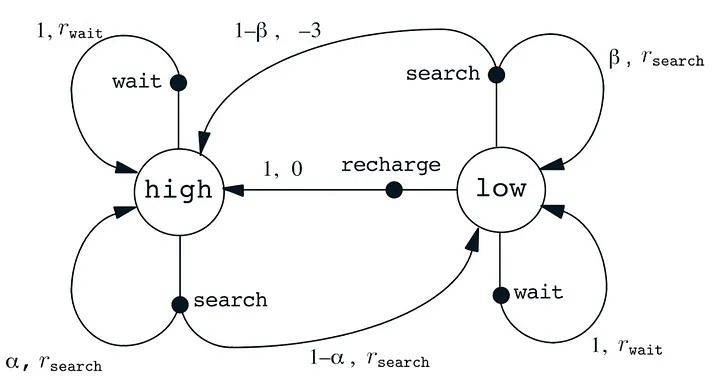
\includegraphics[height=5cm]{Pictures/deep-reinforcement-learning/eg1_mdp_fig.jpg}
            \caption{An example of a transition diagram}
        \end{figure}
    \end{minipage}
    \hfill
    \begin{minipage}{0.35\linewidth}
        \begin{figure}[H]
            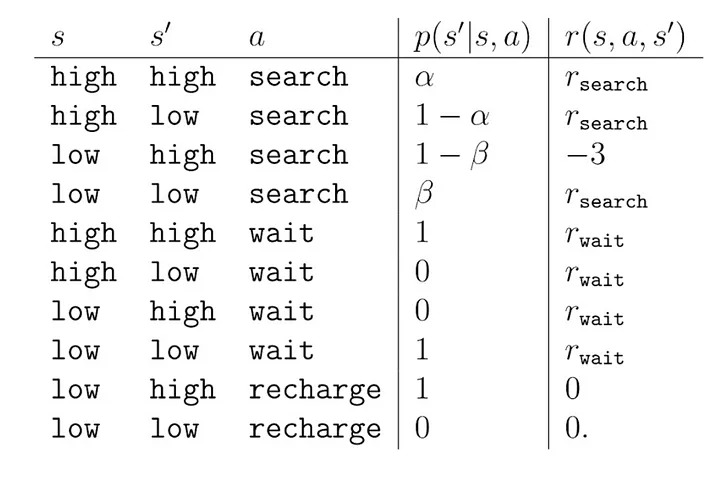
\includegraphics[height=5cm]{Pictures/deep-reinforcement-learning/eg1_mdp_table.jpg}
            \caption{An example of a transition probability table}
        \end{figure}
    \end{minipage}
\end{table}

A transition diagram is simply a graph that tells you, the agent, what are the possible actions at each state. It can sometimes have the probability of taking each action, and what are the rewards for taking each action.\\
In the above example, first row - We can see how in this environment we can go from the state "$high$" to the state "$high$" by taking the action "$search$" . We can also see that we have a probability of "$\alpha$" of moving the state "$high$" after being in state "$high$" and taking action "$\alpha$". Lastly, we can see that the reward that we will get doing such, will be "$r_{search}$".


\section{Bellman equation \cite{medium-introduction-to-reinforcement-learning-rl-part-3-finite-markov-decision-processes-51e1f8d3ddb7}}
\begin{align*}
v_\pi(s)  &= \mathbb{E}_\pi [G_t \mid S_t = s] \\ 
    &= \mathbb{E}_\pi [R_{t+1} + \gamma V(S_{t+1}) \mid S_t = s] \\ 
    % &= \mathbb{E}_\pi \left[ \sum_{k=0}^{\infty} \gamma^k R_{t+k+1} \bigg| S_t = s \right] \\
    &= \mathbb{E}_\pi \left[ R_{t+1} + \gamma \sum_{k=0}^{\infty} \gamma^k R_{t+k+2} \bigg| S_t = s \right] \hspace{3cm} \left(V(S_{t}) = \sum_{k=0}^{\infty} \gamma^k R_{t+k+1} \right) \\ 
    &= \sum_a \pi(a \mid s) \sum_{s'} \sum_r p(s', r \mid s, a) \left[ r + \gamma \mathbb{E}_\pi \left[ \sum_{k=0}^{\infty} \gamma^k R_{t+k+2} \bigg| S_{t+1} = s' \right] \right] \\ 
    &= \sum_a \pi(a \mid s) \sum_{s', r} p(s', r \mid s, a) \left[ r + \gamma v_\pi(s') \right] 
\end{align*}

\begin{enumerate}
    \item $\pi(a|s)$ is the probability of taking action "$a$" in state "$s$" under policy $\pi$
    \item It expresses a relationship between the value of a state $S$, and the values of the next state $S'$, following policy $\pi$.
    \item Think about it as “the value of a given a state (where you currently are) depends on what following states are possible”.
\end{enumerate}

\begin{table}[H]
    \begin{minipage}{0.45\linewidth}
        \begin{figure}[H]
            \centering
            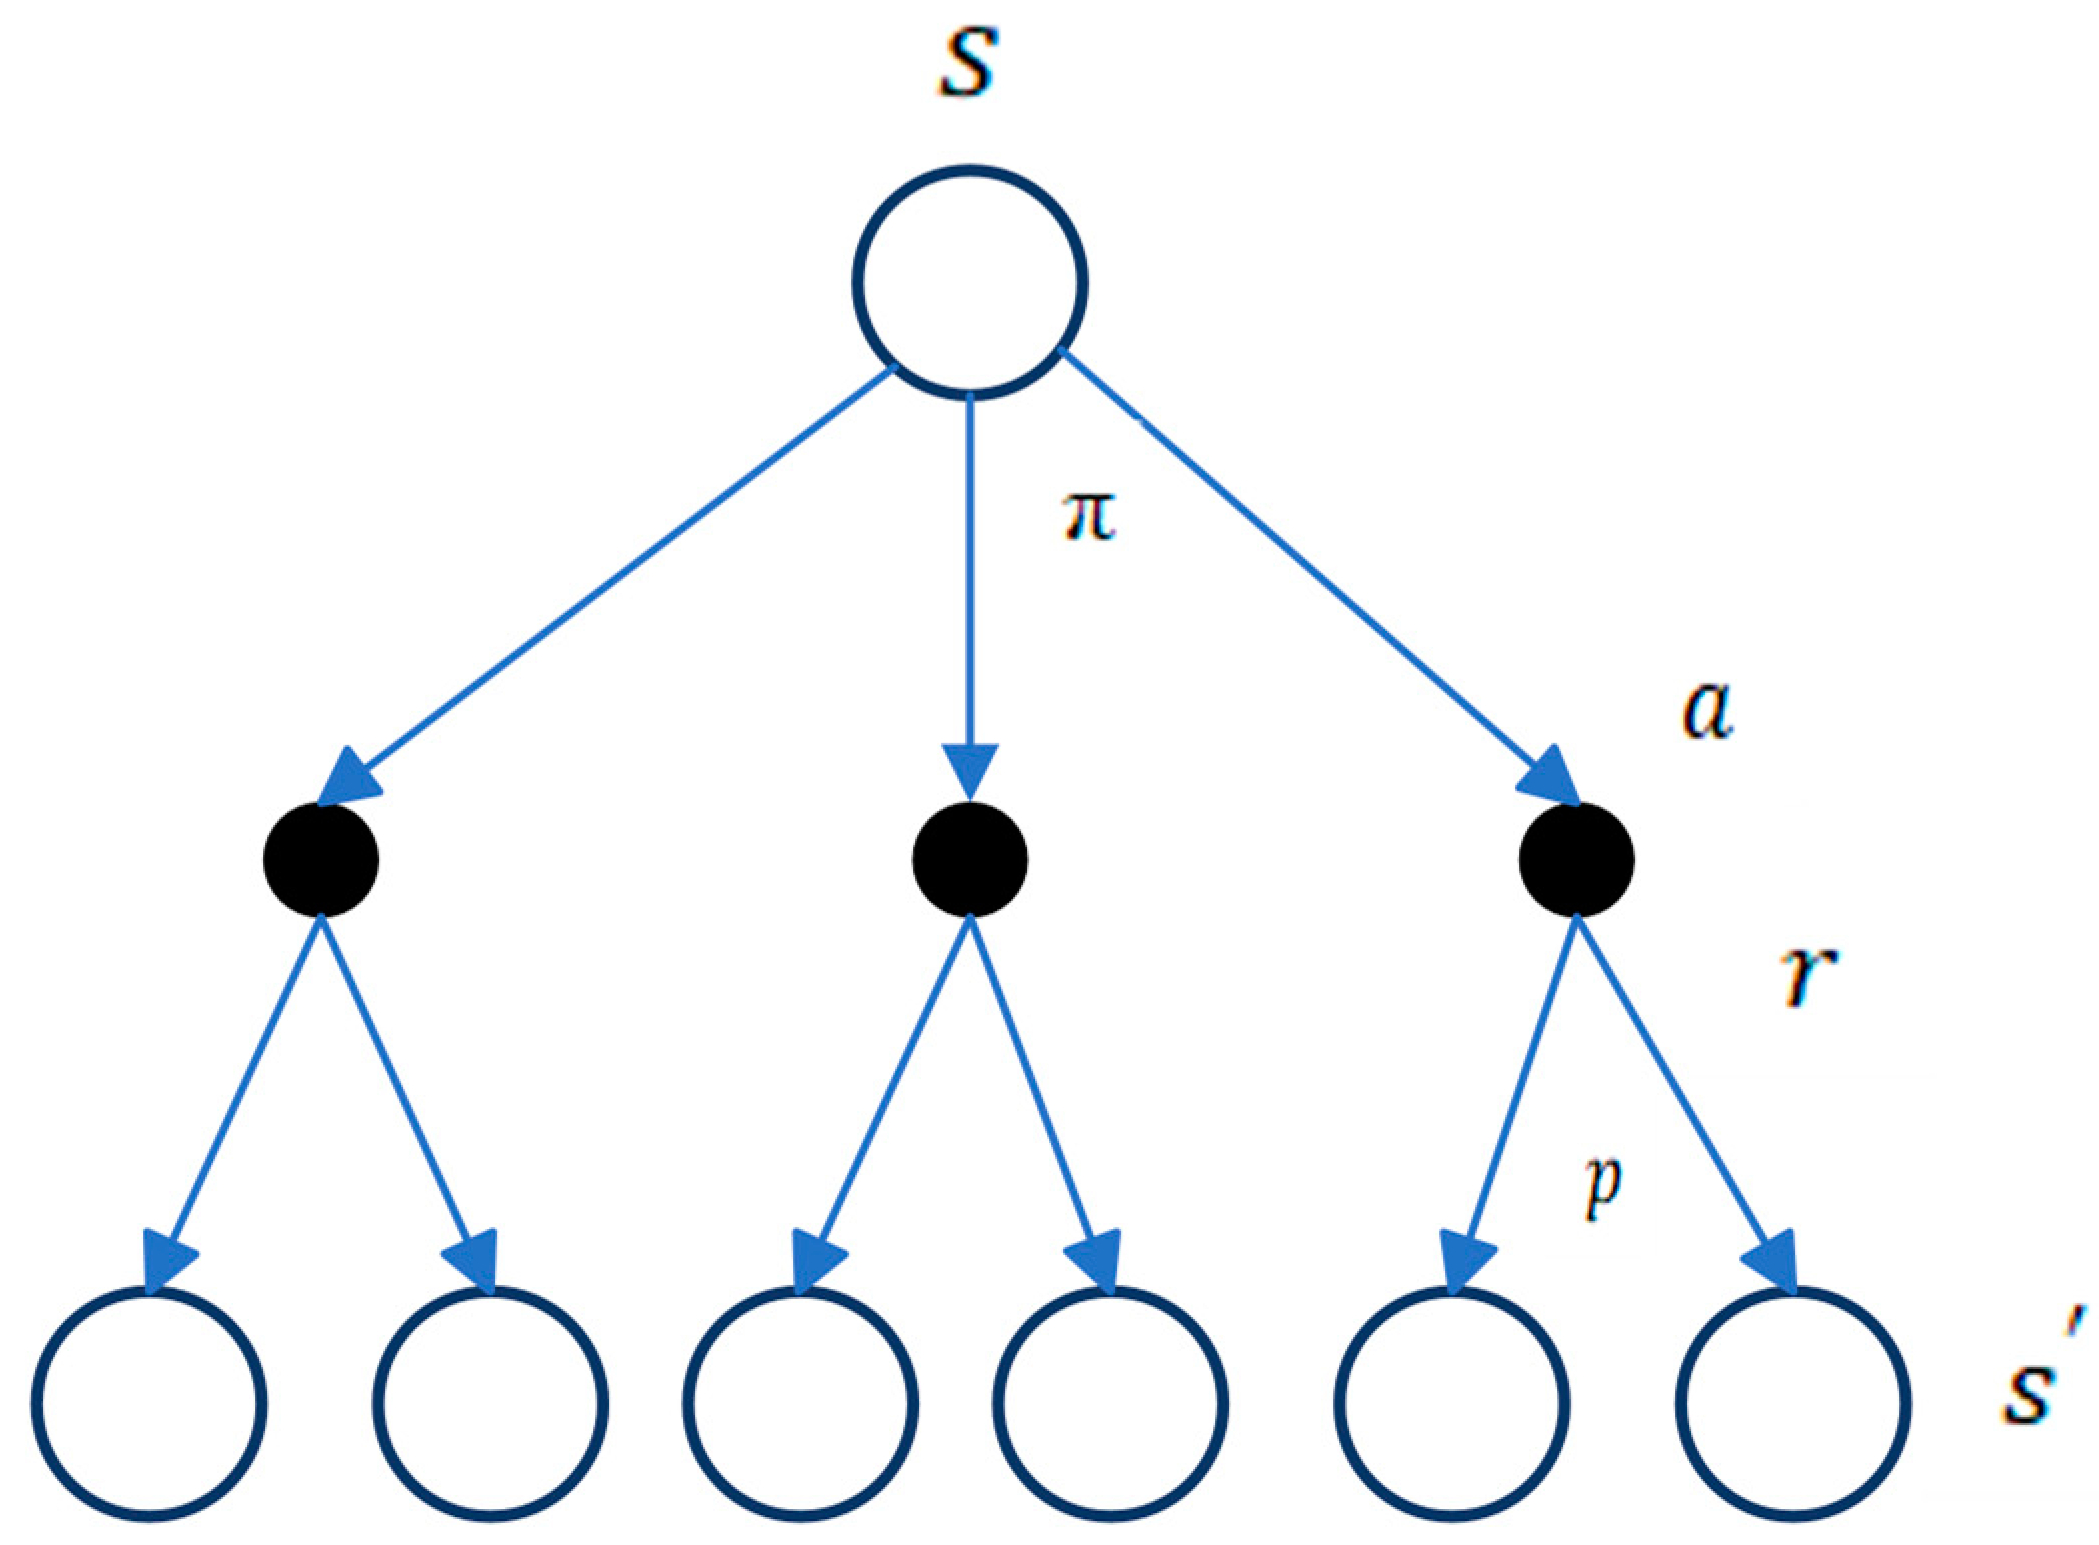
\includegraphics[height=4.5cm]{Pictures/deep-reinforcement-learning/drl-backup-diagram_v-pi.jpg}
            \caption{Backup diagram for $v_\pi$}
        \end{figure}
    \end{minipage}
    \hfill
    \begin{minipage}{0.45\linewidth}
        We’re basically computing the expected value of the state $S$ (top node - our current state) using all the next states (bottom nodes) it can transition into.\\
        We call those diagram \textbf{backup diagrams} because they show how the update or backup operations work. We transfer information back to a state from its possible following states.
    \end{minipage}
\end{table}

Bellman equation for the value of a state:
\begin{align*}
    v_\pi(s) &\doteq \mathbb{E}_\pi [G_t \mid S_t = s] \\
    &= \mathbb{E}_\pi [R_{t+1} + \gamma G_{t+1} \mid S_t = s]
\end{align*}

\section{Optimal Value Functions \cite{medium-introduction-to-reinforcement-learning-rl-part-3-finite-markov-decision-processes-51e1f8d3ddb7}}

The Bellman optimality equations are a way of solving for the optimal value of states.


The optimal value of a state is denoted by $V_*(s)$



\begin{align*}
v_*(s) &= \max_{a \in {A}(s)} q_{\pi_*}(s, a) \\
    &= \max_a \mathbb{E}_{\pi_*} [G_t \mid S_t = s, A_t = a] \\
    &= \max_a \mathbb{E}_{\pi_*} \left[ \sum_{k=0}^{\infty} \gamma^k R_{t+k+1} \mid S_t = s, A_t = a \right] \\
    &= \max_a \mathbb{E}_{\pi_*} \left[ R_{t+1} + \gamma \sum_{k=0}^{\infty} \gamma^k R_{t+k+2} \mid S_t = s, A_t = a \right] \\
    &= \max_a \mathbb{E} [R_{t+1} + \gamma v_*(S_{t+1}) \mid S_t = s, A_t = a]
\end{align*}
\[
    v_*(s) = \max_{a \in {A}(s)} \sum_{s',r} p(s', r \mid s, a) \left[ r + \gamma v_*(s') \right]
\]

\begin{align*}
    q_*(s,a) &= \mathbb{E}[R_{t+1} + \gamma \max_{a'} q_*(S_{t+1},a') | S_t=s,A_t=a] \\
    &= \sum_{s',r} p(s',r | s,a) \left[ r + \gamma \max_{a'} q_*(s',a') \right]
\end{align*}

Quite similar to before, but now we’re taking "$\max(a)$", meaning, the action with the best reward for each state in order to maximize the reward.

The optimal policy $\pi_*$ tells us what’s the best course of actions.






















































